%======================================================================
\subsection{MOD-06 plan: sheet metal from the bundled SheetMetal add-on (23 Oct 2026, approved 24 Oct)}\label{sec:mod06-plan}
%======================================================================

\eref{MOD-06} gives Vector Labs sheet metal by bundling the open-source SheetMetal add-on (\code{shaise/FreeCAD\_SheetMetal})
rather than writing a new one. This plan says what was tested in this build, the theory the flat pattern rests on, how
the add-on is bundled and shown as the \emph{Design $\rightarrow$ Sheet Metal} tab, the per-vault rules, and the outputs
(flat DXF and bend table) that tie it to \eref{MFG-03} and \eref{DRW-07}.

\paragraph{Your answers (23 Oct).}
\begin{center}
\small
\begin{tabularx}{\linewidth}{@{}lX@{}}
\toprule
Question & Answer\\
\midrule
Build or bundle & \textbf{Bundle} SheetMetal: base wall, flanges, relief, unfold, K-factor tables.\\
Where in the UI & The \textbf{Design $\rightarrow$ Sheet Metal} tab (it was left out of \file{workspaces.json} because the
  add-on was not installed).\\
Rules & \textbf{Per vault}: material, thickness, K-factor, bend radius, stored next to the vault's other settings
  (\file{vault\_setup.py}, \file{drawing\_standards.py}).\\
Outputs & \textbf{Flat DXF and a bend table} (\eref{MFG-03}, \eref{DRW-07}).\\
\bottomrule
\end{tabularx}
\end{center}

%----------------------------------------------------------------------
\subsubsection*{1. What was tested (23 Oct)}

SheetMetal~0.8.26 (commit \code{cbf6595}, 17 Oct 2026) was cloned into a scratch folder and loaded into this build
(FreeCAD~1.1.4-bw, Python~3.11) with FreeCAD's own \code{-M <folder>} switch, on a copy of your configuration. Nothing
was installed into your \file{Mod} folder. The add-on's new unfolder needs \code{networkx}, which this build's Python
does not have; a scratch copy of networkx~3.5 was passed with \code{-P}.
\begin{center}
\small
\begin{tabularx}{\linewidth}{@{}Xl@{}}
\toprule
Check & Result\\
\midrule
Add-on's own unit tests (\code{FreeCADCmd -t TestSheetMetal}) & 7 of 7 pass, 0.22\,s\\
Commands registered without switching workbench (import of its 16 command modules) & 19 \code{SheetMetal\_*} commands\\
Bracket A: base plate $40\times30$ + one flange (\emph{Make Wall}, Outer Sharp, Material Inside) & valid solid,
  3\,029.386\,mm$^3$\\
Bracket B: one base wall from an open L sketch & same solid, same volume\\
Unfold at $K=0.44$, both brackets & flat 67.1783\,mm; formula 67.1783\,mm; error $<10^{-4}$\,mm\\
K sweep 0.30, 0.33, 0.40, 0.44, 0.50 & every flat equals the formula to $10^{-5}$\,mm\\
Flange, unfold, DXF times & 0.024\,s, 0.005\,s, 0.003\,s\\
DXF from the add-on's sketches (GUI, separate layers) & layers named after sketches; 17 lines, 8 arcs (label text as geometry)\\
Bend data without the GUI (\code{getUnfold}) & one bend: $+90^\circ$, $R=2$, line 30\,mm; flat area 2\,015.35\,mm$^2$\\
\bottomrule
\end{tabularx}
\end{center}
The acceptance of \eref{MOD-06} (\emph{the bracket of Figure~\ref{fig:sheet} unfolds to the bend-allowance length
within 0.01\,mm}) is therefore already met by the add-on itself: the analytic check in the roadmap and the add-on agree
to the fourth decimal.

\begin{figure}[!htbp]
\centering
\begin{minipage}[b]{0.36\linewidth}\centering
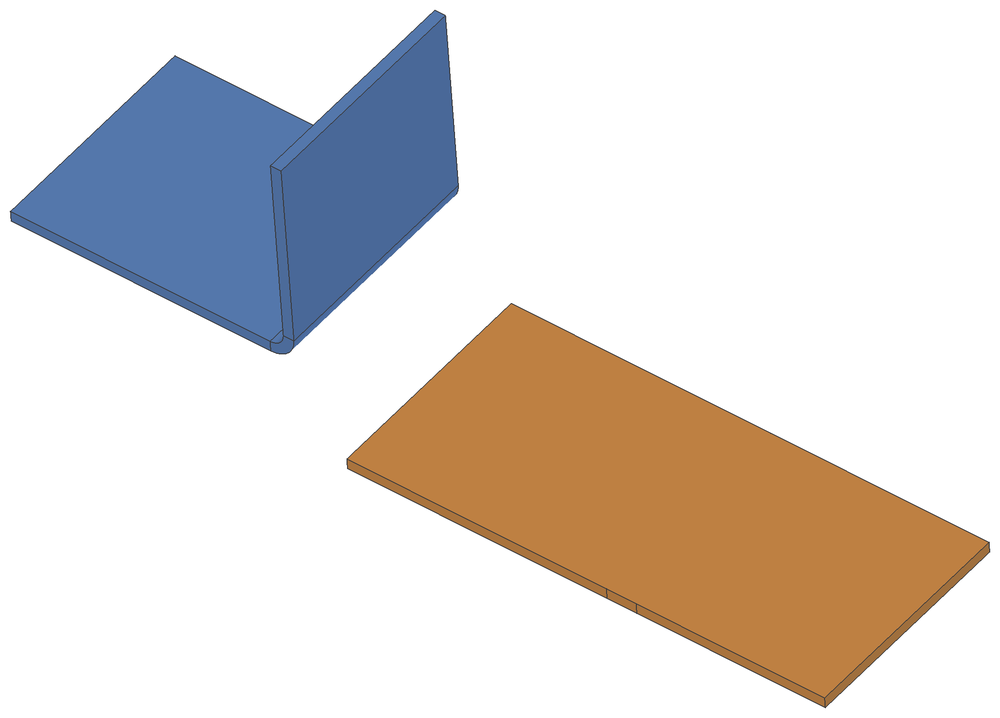
\includegraphics[width=\linewidth]{fig/mod06_bracket.png}\\[-2pt]{\footnotesize (a)}
\end{minipage}\hfill
\begin{minipage}[b]{0.6\linewidth}\centering
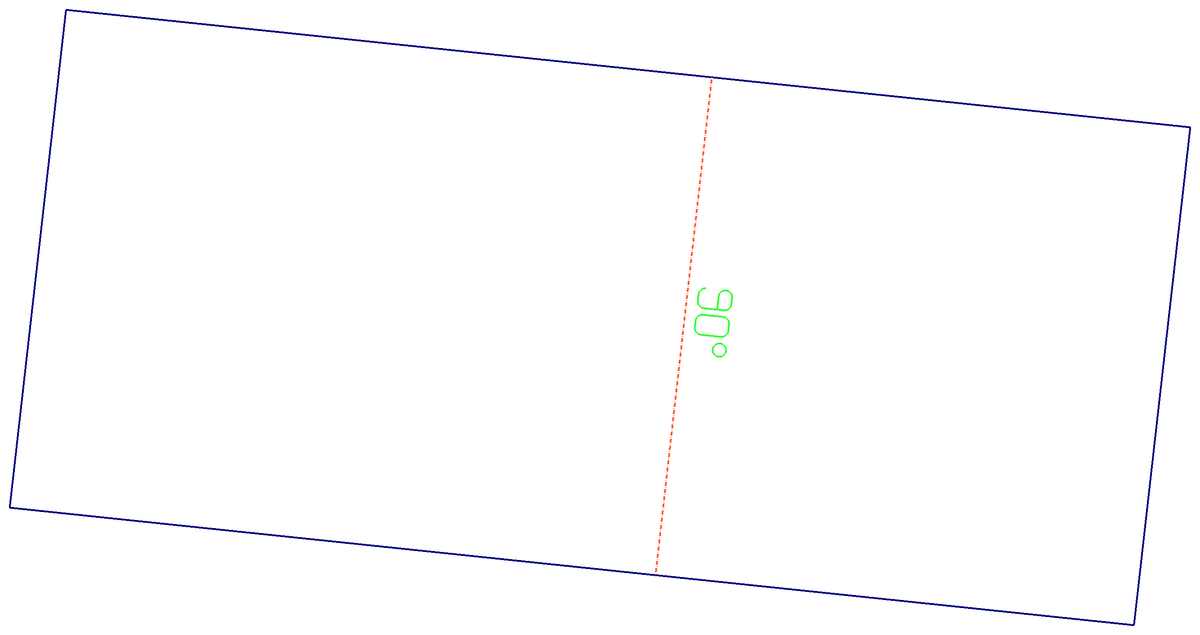
\includegraphics[width=\linewidth]{fig/mod06_flat_sketch.png}\\[-2pt]{\footnotesize (b)}\\[6pt]
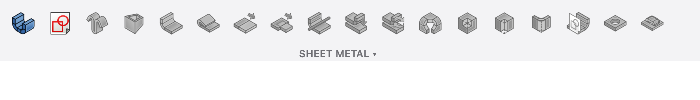
\includegraphics[width=\linewidth]{fig/mod06_toolbar.png}\\[-2pt]{\footnotesize (c)}
\end{minipage}
\caption{The spike in this build (light theme). (a)~Bracket A (blue) and its flat (orange), $T=1.5$, $R=2$, $K=0.44$.
(b)~The unfold sketch the add-on makes in the GUI: outline, bend line (dash-dot) and the angle label.
(c)~The add-on's own toolbar, 18 commands, today reachable only as a ``More workbenches'' tab.}
\label{fig:mod06-spike}
\end{figure}

\paragraph{Four findings to fix or work around.}
\begin{enumerate}[nosep]
  \item \textbf{K-factor tables interpolate wrongly.} \code{BendAllowanceCalculator.get\_k\_factor} (new unfolder) walks
        the table with \code{while r\_over\_t <= values[i]}, so it always uses the first segment and extrapolates. With
        the table $R/T = 1, 2, 3, 5 \mapsto K = 0.30, 0.40, 0.45, 0.50$ it returns 0.45 at $R/T=2.5$ (correct 0.425) and
        0.60 at $R/T=4$ (correct 0.475). Single-value K and two-row tables are right. Fix: one-line patch, offered
        upstream.
  \item \textbf{Unfold sketches need the GUI.} With \emph{Generate sketch} and either \emph{separate layers} or
        \emph{bend labels}, the unfold fails without a GUI (\code{ViewObject} is \code{None} in
        \code{getUnfoldSketches}). The release package (\eref{MFG-04}) runs headless, so our DXF writer reads the bend
        data from \code{getUnfold} instead (that works headless, row above), and the upstream guard is offered as a patch.
  \item \textbf{The add-on's DXF is not a shop DXF.} Its layers are sketch names, bend labels are line geometry, and
        there is no up/down for bends. \eref{MFG-03} needs \code{CUT}, \code{BEND\_UP}, \code{BEND\_DOWN},
        \code{ETCH}; we write those ourselves (step~6).
  \item \textbf{Licence headers are mixed} (section~4): 8 of 37 Python files still carry GPL-2.0-or-later headers.
\end{enumerate}

%----------------------------------------------------------------------
\subsubsection*{2. Theory: bend allowance, bend deduction and the K-factor}

\begin{figure}[!htbp]
\centering
\begin{tikzpicture}[scale=0.62,>=Stealth]
  \def\R{2}\def\T{1.5}\def\K{0.44}
  % material
  \fill[bwblue!18] (-7,-\R-\T) -- (0,-\R-\T) arc (-90:0:\R+\T) -- (\R+\T,6) -- (\R,6) -- (\R,0) arc (0:-90:\R) -- (-7,-\R) -- cycle;
  \draw[bwblue,thick] (-7,-\R-\T) -- (0,-\R-\T) arc (-90:0:\R+\T) -- (\R+\T,6);
  \draw[bwblue,thick] (-7,-\R) -- (0,-\R) arc (-90:0:\R) -- (\R,6);
  % neutral fibre
  \draw[bworange,thick,dashed] (-7,-\R-\K*\T) -- (0,-\R-\K*\T) arc (-90:0:\R+\K*\T) -- (\R+\K*\T,6);
  \node[bworange,font=\scriptsize,anchor=west] at (\R+\T+0.1,5.3) {neutral fibre, $R+KT$};
  % tangent lines
  \draw[bwgrey,densely dotted] (0,-\R-\T-0.8) -- (0,0.6);
  \draw[bwgrey,densely dotted] (-0.6,0) -- (\R+\T+0.9,0);
  % mould lines and virtual sharp
  \draw[bwgrey,dashed] (0,-\R-\T) -- (\R+\T+0.0,-\R-\T) -- (\R+\T,0);
  \fill[bwred] (\R+\T,-\R-\T) circle (2.2pt);
  \node[bwred,font=\scriptsize,anchor=north west] at (\R+\T,-\R-\T) {virtual sharp};
  % radius
  \fill (0,0) circle (1.5pt);
  \draw[->] (0,0) -- (-135:\R) node[midway,above left,font=\scriptsize] {$R$};
  % thickness
  \draw[<->] (-5.5,-\R) -- (-5.5,-\R-\T) node[midway,left,font=\scriptsize] {$T$};
  % OSSB
  \draw[<->] (0,-\R-\T-0.55) -- (\R+\T,-\R-\T-0.55) node[midway,below,font=\scriptsize] {$\mathit{OSSB}$};
  % angle
  \draw[->,bwdark] (\R+\T+1.6,-0.5) arc (-30:40:1.0) node[right,font=\scriptsize] {$\theta=90^\circ$};
  \node[font=\scriptsize,bwblue] at (-4,-\R-\T-0.5) {flange 1};
  \node[font=\scriptsize,bwblue,rotate=90] at (\R+\T+0.5,3.5) {flange 2};
\end{tikzpicture}
\caption{A bend in section. The neutral fibre keeps its length while bending; it lies at $R+KT$ from the bend axis.
The outside setback $\mathit{OSSB}$ runs from a tangent line to the virtual sharp where the outer mould lines meet.}
\label{fig:mod06-bend}
\end{figure}

Bending stretches the outer fibres and compresses the inner ones; one fibre, the \emph{neutral fibre}, keeps its length.
The K-factor places it: $K = t/T$, where $t$ is its distance from the inner surface, $0 < K \le 0.5$. The flat length of
the bend zone is the neutral fibre's arc, the \textbf{bend allowance}
\[
  \mathit{BA} = \theta\,(R + K\,T),
\]
with $\theta$ the bend angle in radians and $R$ the inner radius. Two equivalent ways to get the flat:
\[
  L_{\text{flat}} = \sum_i \ell_i + \sum_j \mathit{BA}_j
  \qquad\text{or}\qquad
  L_{\text{flat}} = \sum_i L_i^{\text{out}} - \sum_j \mathit{BD}_j ,
\]
\[
  \mathit{BD} = 2\,\mathit{OSSB} - \mathit{BA},\qquad \mathit{OSSB} = \tan\tfrac{\theta}{2}\,(R+T),
\]
where $\ell_i$ are the straight lengths between tangent lines and $L_i^{\text{out}}$ the outside (mould-line)
dimensions a drawing gives. For the bracket ($T=1.5$, $R=2$, $K=0.44$, $\theta=\pi/2$):
$\mathit{BA}=\tfrac{\pi}{2}(2+0.66)=4.178$, $\mathit{OSSB}=3.5$, $\mathit{BD}=7-4.178=2.822$, and
$L_{\text{flat}} = 40+30-2.822 = 67.178$\,mm, as the add-on computed.

\paragraph{Sensitivity.} $\partial L_{\text{flat}}/\partial K = \theta T$, here $2.356$\,mm per unit of K, so an error of
0.01 in K moves the flat by 0.024\,mm per bend. The sweep in section~1 shows exactly this slope
($66.8485 \rightarrow 67.3197$ for $K = 0.30 \rightarrow 0.50$). The rule table matters more than the unfolder.

\paragraph{Typical K-factors} (ANSI convention, $0 \le K \le 0.5$; published rules of thumb, to be replaced by the
shop's numbers):
\begin{center}
\small
\begin{tabular}{@{}lccc@{\qquad}ccc@{}}
\toprule
 & \multicolumn{3}{c}{Air bending} & \multicolumn{3}{c}{Bottoming}\\
$R$ vs $T$ & Aluminium & Mild steel & Stainless & Aluminium & Mild steel & Stainless\\
\midrule
$R < T$ & 0.33 & 0.38 & 0.40 & 0.42 & 0.44 & 0.46\\
$T \le R \le 3T$ & 0.40 & 0.43 & 0.45 & 0.46 & 0.47 & 0.48\\
$R > 3T$ & 0.50 & 0.50 & 0.50 & 0.50 & 0.50 & 0.50\\
\bottomrule
\end{tabular}
\end{center}
The German convention (DIN~6935) uses $k = 2K$ ($0\ldots1$) and for steel $k = 0.65 + \tfrac12\log_{10}(R/T)$ when
$R/T<5$. For the bracket ($R/T=1.33$) that is $k=0.712$, $K=0.356$, a flat 0.198\,mm shorter than with $K=0.44$; the
add-on accepts either convention (\code{KFactorStandard} \code{ansi}/\code{din}). Two more rules of thumb go into the
rules: the bend relief is at least $T$ wide and $R+T$ deep, and the shortest flange is about $2.5\,T + R$ so the
part sits on the die.

%----------------------------------------------------------------------
\subsubsection*{3. Per-vault sheet-metal rules}

A rule is one line of a table the vault owns, like Fusion's sheet-metal rules:
\begin{center}
\small
\begin{tabularx}{\linewidth}{@{}lllllllX@{}}
\toprule
Rule & Material & $T$ & $R$ & $K$ & Relief $w\times d$ & Min flange & Note\\
\midrule
AL5052-1.5 & Al 5052-H32 & 1.5 & 1.5 & 0.40 & $1.5\times3.0$ & 5.25 & default\\
CRS-16ga & Steel CR 1008 & 1.52 & 1.52 & 0.43 & $1.52\times3.0$ & 5.3 & gauge as alias\\
SS304-1.2 & Stainless 304 & 1.2 & 1.2 & 0.45 & $1.2\times2.4$ & 4.2 & \\
\bottomrule
\end{tabularx}
\end{center}

\begin{itemize}[nosep]
  \item \textbf{Storage.} \file{<vault>/sheet\_metal\_rules.json}, format \code{bruceworx.sheet-metal-rules}, read and
        written by a new FreeCAD-free module \file{bruceworx/sheetmetal\_rules.py} in \file{addons/BruceWorx} with the
        same shape as \file{drawing\_standards.py} (\code{load}, \code{validate}, \code{save}, \code{csv\_rows}). The
        vault's CSV gains a \code{sheetmetal} table, so rules can be edited in a spreadsheet with the other settings.
        Rules are added and retired, never deleted, so old parts keep their rule. The other agent owns
        \file{vault\_setup.py} and \file{drawing\_standards.py}; this plan only adds the table name to the CSV parser.
  \item \textbf{Editing.} A \emph{Sheet metal} page in Vault Settings (table with add, duplicate, retire), and the
        Create Vault wizard seeds the three rules above (question~4).
  \item \textbf{Applying.} A part gets a rule from the \emph{Sheet-metal rule} command (also offered when the first base
        wall is made). The rule's values go into a per-document \code{App::VarSet} named \code{SheetMetalRule}, and the
        add-on's properties are bound to it by expressions: \code{Thickness}, \code{Radius}, \code{radius},
        \code{reliefw}, \code{reliefd} on every wall and \code{KFactor} on the unfold. Changing the rule updates the
        whole part in one recompute, and a feature can still override a value by breaking its expression.
  \item \textbf{One K per rule.} A rule fixes $T$ and $R$, so $R/T$ is fixed and one K is exact; the add-on's
        lookup tables (and their bug) are not needed. A table per material by $R/T$ can come later (question~3).
  \item \textbf{Part properties.} The rule name, material and thickness are written to the part's properties
        (\code{Material}, \code{Stock} = \code{"Sheet 1.5 Al 5052-H32"}) so the BOM and the title block show them.
\end{itemize}

%----------------------------------------------------------------------
\subsubsection*{4. Bundling, licences and notices}

\paragraph{How it is shipped.} The same pattern as \file{addons/BruceWorx} (installed as \file{Mod/BruceWorxHooks}):
\begin{itemize}[nosep]
  \item A vendored copy in \file{package/bruceworx/vendor/SheetMetal/}, pinned to an upstream commit recorded in
        \file{VENDOR.txt}, with our few patches as separate \code{[BW]} commits so each update is a rebase.
  \item \file{package/bruceworx/vendor/CMakeLists.txt}: \code{option(BUILD\_BW\_SHEETMETAL ... ON)} next to
        \code{BUILD\_BW\_HOOKS} in \file{src/Mod/CMakeLists.txt}; \code{fc\_copy\_sources} into
        \file{<build>/Mod/SheetMetal} and \code{INSTALL(DIRECTORY ... DESTINATION Mod/SheetMetal)} excluding
        \file{SMTests}, \file{.github} and the translation tools. Unlike the hooks add-on, \file{package.xml}
        \emph{is} installed: it names the workbench.
  \item \textbf{networkx} goes into \file{pixi.toml} (\code{networkx = ">=3.4.2,<3.6"}; 3.6 and later need Python~3.12),
        so it lands in the install prefix and \file{make-dmg.sh} copies it into the \file{.dmg} with everything else.
  \item \textbf{Off switch.} Preferences $\rightarrow$ BruceWorx $\rightarrow$ \emph{Sheet metal add-on} (default on)
        adds \code{SheetMetal} to FreeCAD's \code{DisabledAddons} list, the mechanism \file{FreeCADInit.py} already
        uses for the Ribbon add-on.
  \item \textbf{A user copy wins.} FreeCAD keys modules by lower-case folder name and loads the user's \file{Mod}
        after the built-in one, so a SheetMetal installed from the Addon Manager replaces ours (FreeCAD prints
        ``2 entries found''). Vector Labs shows this once in the status bar (question~1).
\end{itemize}

\paragraph{Licence findings.}
\begin{center}
\small
\begin{tabularx}{\linewidth}{@{}lX@{}}
\toprule
Item & Finding\\
\midrule
SheetMetal \file{LICENSE}, \file{package.xml} & LGPL-2.1 text; \code{LGPL-2.1-or-later} (relicensed from GPL-3 in
  v0.4.00, Jan 2024)\\
File headers & 25 files LGPL-2.1-or-later; \textbf{8 files GPL-2.0-or-later}: \file{SheetMetalCmd.py} (the flange,
  2\,377 lines), \file{ExtrudedCutout.py}, \file{SheetMetalCornerReliefCmd.py}, \file{SheetMetalFromSolid.py},
  \file{SheetMetalHem.py}, \file{SheetMetalJunction.py}, \file{SheetMetalSketch.py}, \file{SheetMetalText.py};
  4 files without a header. The 2024 relicence commit did not touch them.\\
networkx~3.5 & BSD-3-Clause\\
Compatibility & LGPL-2.1-or-later FreeCAD may be combined with GPL-2.0-or-later code: the combination is then
  distributed under the GPL, whose main duty, the complete source, Vector Labs already meets (\eref{FND-04}: a source
  archive with every release; Python is shipped as source). Nothing here blocks the internal \file{.dmg}.\\
\bottomrule
\end{tabularx}
\end{center}
Notices (\eref{FND-04}): a \emph{Third-party components} section in \file{NOTICE} lists SheetMetal (commit, licence,
``some files GPL-2.0-or-later'') and networkx, and their licence files are installed under
\file{share/doc/BruceWorx/third-party/}. We also open an upstream issue asking for the eight headers to be brought in
line with the README. (This is an engineering reading, not legal advice.)

%----------------------------------------------------------------------
\subsubsection*{5. The Sheet Metal tab}

In \file{workspaces.json} terms, a new tab in the Design workspace after \emph{Surface} (Fusion's order: Solid,
Surface, Mesh, Sheet Metal, Utilities). The 16 command modules are added to \code{"load"}, so the commands register
without leaving Part Design (tested: all 19 appear while Part Design stays active). The tab carries a new
\code{"requires": "SheetMetal"} key: \file{bruceworx\_workspaces.py} hides the tab when the add-on is missing or
switched off, which is why it was left out before.
\begin{lstlisting}[language={}]
{ "name": "Sheet Metal", "requires": "SheetMetal", "groups": [
  { "caption": "Create",
    "commands": ["SheetMetal_AddBase", "SheetMetal_AddWall", "SheetMetal_AddFoldWall",
                 "SheetMetal_Extrude", "SheetMetal_AddHem"],
    "more": ["SheetMetal_BaseShape", "SheetMetal_FromSolid", "SheetMetal_ExtendBySketch",
             "SheetMetal_AddBend", "SheetMetal_NewSketch"] },
  { "caption": "Modify",
    "commands": ["SheetMetal_AddRelief", "SheetMetal_AddCornerRelief",
                 "SheetMetal_AddJunction", "SheetMetal_AddCutout"],
    "more": ["SheetMetal_SketchOnSheet", "SheetMetal_Forming"] },
  { "caption": "Flat",
    "commands": ["SheetMetal_Unfold", "BruceWorx_ExportFlat"],
    "more": ["SheetMetal_UnfoldUpdate", "SheetMetal_UnattendedUnfold"] },
  { "caption": "Rules",
    "commands": ["BruceWorx_SheetMetalRule"], "more": ["BruceWorx_SheetMetalRules"] } ] }
\end{lstlisting}
Three commands are ours:
\begin{itemize}[nosep]
  \item \code{BruceWorx\_ExportFlat} writes the shop DXF and the bend table (next section);
  \item \code{BruceWorx\_SheetMetalRule} picks the part's rule;
  \item \code{BruceWorx\_SheetMetalRules} opens the vault's rule table.
\end{itemize}
The add-on's own task panels are kept (figure~\ref{fig:mod06-panel}); they already have the Fusion-like fields.

\begin{figure}[!htbp]
\centering
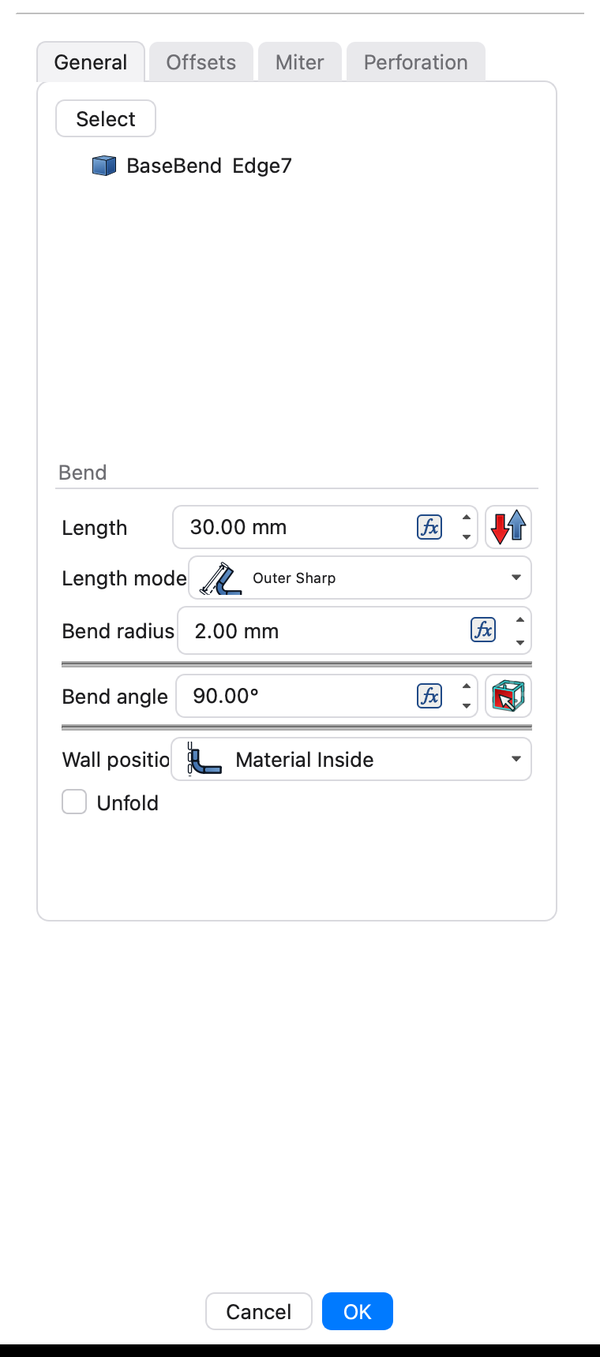
\includegraphics[width=0.3\linewidth]{fig/mod06_wall_panel.png}\hspace{1.5em}
\begin{minipage}[b]{0.55\linewidth}
\caption{The add-on's \emph{Make Wall} (flange) panel in this build, light theme: length mode (Leg, Outer Sharp, Inner
Sharp, Tangential), bend radius, angle, wall position, and tabs for offsets, mitre and perforation. With a rule applied,
the radius field shows the expression to \code{SheetMetalRule.Radius}.}
\label{fig:mod06-panel}
\end{minipage}
\end{figure}

%----------------------------------------------------------------------
\subsubsection*{6. Outputs: the shop DXF (MFG-03) and the bend table (DRW-07)}

\begin{figure}[!htbp]
\centering
\begin{tikzpicture}[scale=0.11,>=Stealth]
  % flat 67.178 x 30, bend zone 36.5 .. 40.678, bend line at its centre
  \draw[very thick,bwdark] (0,0) rectangle (67.178,30);
  \fill[bwblue!10] (36.5,0) rectangle (40.678,30);
  \draw[bwblue,dashed,thick] (38.589,-2) -- (38.589,32);
  \draw[bwgrey,densely dotted] (36.5,0) -- (36.5,30) (40.678,0) -- (40.678,30);
  \node[font=\scriptsize,bwdark,anchor=north west] at (1,29) {CUT};
  \node[font=\scriptsize,bwblue,anchor=south] at (38.589,32) {BEND\_UP 90$^\circ$ R2};
  \node[font=\scriptsize,bwred] at (18,10) {BW-01-01001 A};
  \node[font=\scriptsize,bwred,anchor=north] at (18,7.8) {ETCH};
  \draw[<->] (0,-4) -- (67.178,-4) node[midway,below,font=\scriptsize] {67.18};
  \draw[<->] (0,-9) -- (36.5,-9) node[midway,below,font=\scriptsize] {36.50};
  \draw[<->] (36.5,-9) -- (40.678,-9) node[midway,below,font=\scriptsize] {BA 4.18};
  \draw[<->] (-4,0) -- (-4,30) node[midway,left,font=\scriptsize] {30};
\end{tikzpicture}
\hfill
\begin{minipage}[b]{0.4\linewidth}
\small
\begin{tabular}{@{}cccccc@{}}
\toprule
Bend & Dir & Angle & $R$ & $K$ & BA\\
\midrule
1 & Up & 90$^\circ$ & 2.00 & 0.44 & 4.18\\
\bottomrule
\end{tabular}\\[4pt]
{\footnotesize Rule AL5052-1.5 (example). Flat $67.18\times30$, $T=1.5$.}\\[18pt]
\end{minipage}
\caption{What \code{BruceWorx\_ExportFlat} produces for the bracket (sketch): \file{P/N-REV.dxf} with layers \code{CUT},
\code{BEND\_UP}/\code{BEND\_DOWN} and \code{ETCH}, and the bend table that the flat-pattern drawing view shows.}
\label{fig:mod06-dxf}
\end{figure}

\begin{itemize}[nosep]
  \item \textbf{DXF (MFG-03).} The flat face comes from \code{SheetMetalNewUnfolder.getUnfold}, which works
        headless. Its outer wire and inner wires go to \code{CUT}; each \code{BendInfo} line goes to \code{BEND\_UP} or
        \code{BEND\_DOWN} by the sign of its angle; the part number and revision go to \code{ETCH} as single-stroke text.
        The writer is a small AutoCAD R12 writer (\code{LINE}, \code{ARC}, \code{CIRCLE}, \code{TEXT}, millimetres),
        the most widely accepted dialect; B-spline edges are approximated by arcs within 0.01\,mm (bi-arc fitting).
        File name \code{P/N-REV.dxf}; \eref{MFG-04} calls the same function when a revision is released.
  \item \textbf{Bend table (DRW-07).} One row per bend in the order of the bend lines from left to right: number,
        direction, angle, inner radius, K, BA. The flat-pattern view is a TechDraw view of the unfold object with the
        bend lines dash-dot and numbered balloons; the table is a TechDraw spreadsheet view, so it updates with the
        model. Fusion and SolidWorks put the same table on the drawing.
  \item \textbf{Check.} A test re-reads the DXF and checks that the \code{CUT} outline's bounding box equals the
        formula flat (0.01\,mm) and that every bend line lies inside its bend zone.
\end{itemize}

%----------------------------------------------------------------------
\subsubsection*{7. Build order and effort}

\begin{center}
\small
\begin{tabularx}{\linewidth}{@{}lXl@{}}
\toprule
\# & Step & Effort\\
\midrule
1 & Vendor SheetMetal (pinned), CMake copy and install, \code{networkx} in \file{pixi.toml}, off switch, NOTICE and
  licence files (\eref{FND-04}) & 1\,d\\
2 & Patches, offered upstream: K-table interpolation, headless unfold sketches; issue about the GPL headers & 0.5\,d\\
3 & Sheet Metal tab in \file{workspaces.json}, \code{"requires"} key, load entries, tab test & 0.5\,d\\
4 & \file{sheetmetal\_rules.py} (pure, with tests), the \code{sheetmetal} CSV table, Vault Settings page, wizard seeds & 1.5\,d\\
5 & \emph{Sheet-metal rule} command: the \code{SheetMetalRule} VarSet, expressions on walls and unfold, part properties & 1.5\,d\\
6 & \code{BruceWorx\_ExportFlat}: R12 DXF writer with layers, arc fitting, headless test on the bracket (MFG-03) & 1.5\,d\\
7 & Flat-pattern drawing view and bend table (DRW-07) & 2\,d\\
8 & Acceptance: bracket within 0.01\,mm, a DXF sent to the laser shop, hook into the release package & 0.5\,d\\
\midrule
 & Total & 9\,d\\
\bottomrule
\end{tabularx}
\end{center}
Steps 1--3 give a usable Sheet Metal tab on day two. Steps 4--5 need only the vault settings that exist today; step~7
follows the drawing work of \eref{DRW-01}.

\paragraph{Risks.} \emph{Upstream churn}: 66 commits in the last twelve months (the add-on is healthy, but things move);
we pin and update deliberately, running its tests and the bracket check each time. \emph{Toponaming}: a flange stores
its base edge by name (\code{BaseBend Edge7}); editing the base sketch can renumber edges and move a flange, as in any
FreeCAD feature on generated faces. \emph{The new unfolder} depends on networkx and is the one we test; the old one stays
reachable through the add-on's own preference. \emph{Licence headers} (section~4) are a paperwork risk, not a technical
one. No upstream FreeCAD code changes: everything is Python and CMake.

%----------------------------------------------------------------------
\paragraph{Your answers to the questions below (24 Oct).} All six as recommended. 1: FreeCAD's rule stays, a newer
SheetMetal from the Addon Manager wins, with a one-time note. 2: upstream is followed \textbf{at every Vector Labs
release}, after its tests and our bracket pass. 3: \textbf{one K per rule} now, the K table per material by $R/T$
later. 4: rules in \textbf{millimetres, gauge as an alias}; a new vault starts with Al~5052-H32 1.0/1.5/2.0/3.0, CR
steel 16/14/12\,ga and stainless 304 1.2/1.5, with the K values of section~2 until the shop gives theirs. 5: a
\textbf{per-vault DXF export profile}, \code{CUT} always, bend layers and \code{ETCH} as switches, all on by default.
6: SheetMetal ships with its eight GPL-2.0-or-later files as they are, noted in \file{NOTICE}, while upstream is asked
to fix the headers. Building started 24 Oct.

\subsubsection*{Questions before MOD-06 starts}

\begin{enumerate}
  \item \textbf{A SheetMetal from the Addon Manager.} If you (or someone) install SheetMetal from the Addon Manager, it
        replaces the bundled one. Keep that rule, or always load the bundled copy?\\
        \emph{Recommendation:} keep FreeCAD's rule (a newer user copy wins) and show a one-time note, so you can try an
        upstream fix without waiting for a Vector Labs build.
  \item \textbf{Updates.} Follow upstream at every Vector Labs release (after its tests and our bracket pass), or only
        when a fix is needed?\\
        \emph{Recommendation:} at every release; the add-on changes often and old pins get hard to rebase.
  \item \textbf{K per rule or K table.} One K per rule (rule fixes $T$ and $R$), or a K table per material by $R/T$?\\
        \emph{Recommendation:} one K per rule now; the table later, once the interpolation fix is upstream.
  \item \textbf{Starting rules.} Which materials and thicknesses should a new vault start with, in millimetres or
        gauge?\\
        \emph{Recommendation:} millimetres, gauge as an alias; seed Al~5052-H32 1.0/1.5/2.0/3.0, CR steel 16/14/12\,ga,
        stainless 304 1.2/1.5, with the K values of section~2 until the shop gives theirs.
  \item \textbf{The shop's DXF.} Which laser shop (or shops)? Some want bend lines on their own layers, some want
        only the cut outline, some want etched part numbers.\\
        \emph{Recommendation:} a per-vault export profile with \code{CUT} always, bend layers and \code{ETCH} as
        switches; default all on.
  \item \textbf{The GPL headers.} Ship SheetMetal with the eight GPL-2.0-or-later files as they are (noted in
        \file{NOTICE}) while upstream is asked to fix the headers?\\
        \emph{Recommendation:} yes; for an internal \file{.dmg} with full source it changes nothing in practice.
\end{enumerate}
